\documentclass[12pt]{article}
\usepackage{graphicx} % Required for inserting images\
\usepackage[margin=1in]{geometry}
\usepackage[T1]{fontenc}
\usepackage{siunitx}
\usepackage{caption}
\usepackage{subcaption}
\usepackage{floatrow}
\usepackage{pgfplots}
\hyphenpenalty=10000
% Table float box with bottom caption, box width adjusted to content
\newfloatcommand{capbtabbox}{table}[][\FBwidth]
\usepackage{float}
\let\origfigure\figure
\let\endorigfigure\endfigure
\renewenvironment{figure}[1][2] {
    \expandafter\origfigure\expandafter[H]
} {
    \endorigfigure
}
\usepackage{titling}



\title{
\includegraphics[width=0.6\linewidth]{weiti.png}\\\\Wstęp do Systemów Wbudowanych\\ Sprawozdanie z Projektu:\\ Sztuczny horyzont}
\author{Jacek Bielski 318492\\ Jakub Wysocki 318596}
\date{Semestr 23Z\\
Terminy zajęć: \\
Piątek 12:15-15:00 (gr. 104)\\
Koordynator przedmiotu: dr hab. inż. prof. uczelni Wojciech Zabłotny \\
Prowadzący: dr inż. Krzysztof Gołofit}
\begin{document}



\maketitle
\newpage

\section{Cel projektu}
        Celem było zrealizowanie sztucznego horyzontu z wykorzystaniem żyroskopu oraz akcelerometru, wyświetlenie go na wyświetlaczu lcd 16x2, a także sygnalizacji dźwiękowej za pomocą sygnału PWM.


\section{Wykorzystywany mikrokontroler oraz peryferia}
        \begin{itemize}
            \item STM32F411-Discovery
                \begin{itemize}
                    \item Żyroskop (I3G4250D)
                    \item Akcelerometr (LSM303AGR)
                    \item generacja PWM (Timer 2 Channel 4)
                \end{itemize}
            \item LCD 16x2 (1602A)
            \item Środowisko: STM32CubeIDE
        \end{itemize}


\section{Schemat blokowy}
  \begin{figure}[H]
\centering
\ffigbox{%
  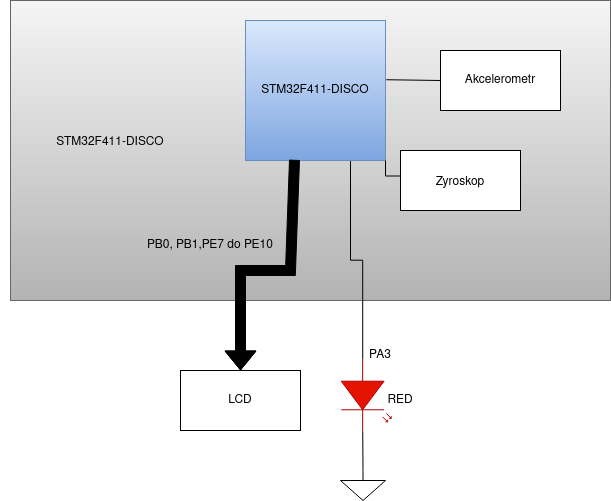
\includegraphics[width=0.6\linewidth]{images/schemat_projektu.png}
}{%
  \caption{Schemat blokowy projektu}%
}
\end{figure}



\begin{figure}[H]
\centering
\ffigbox{%
  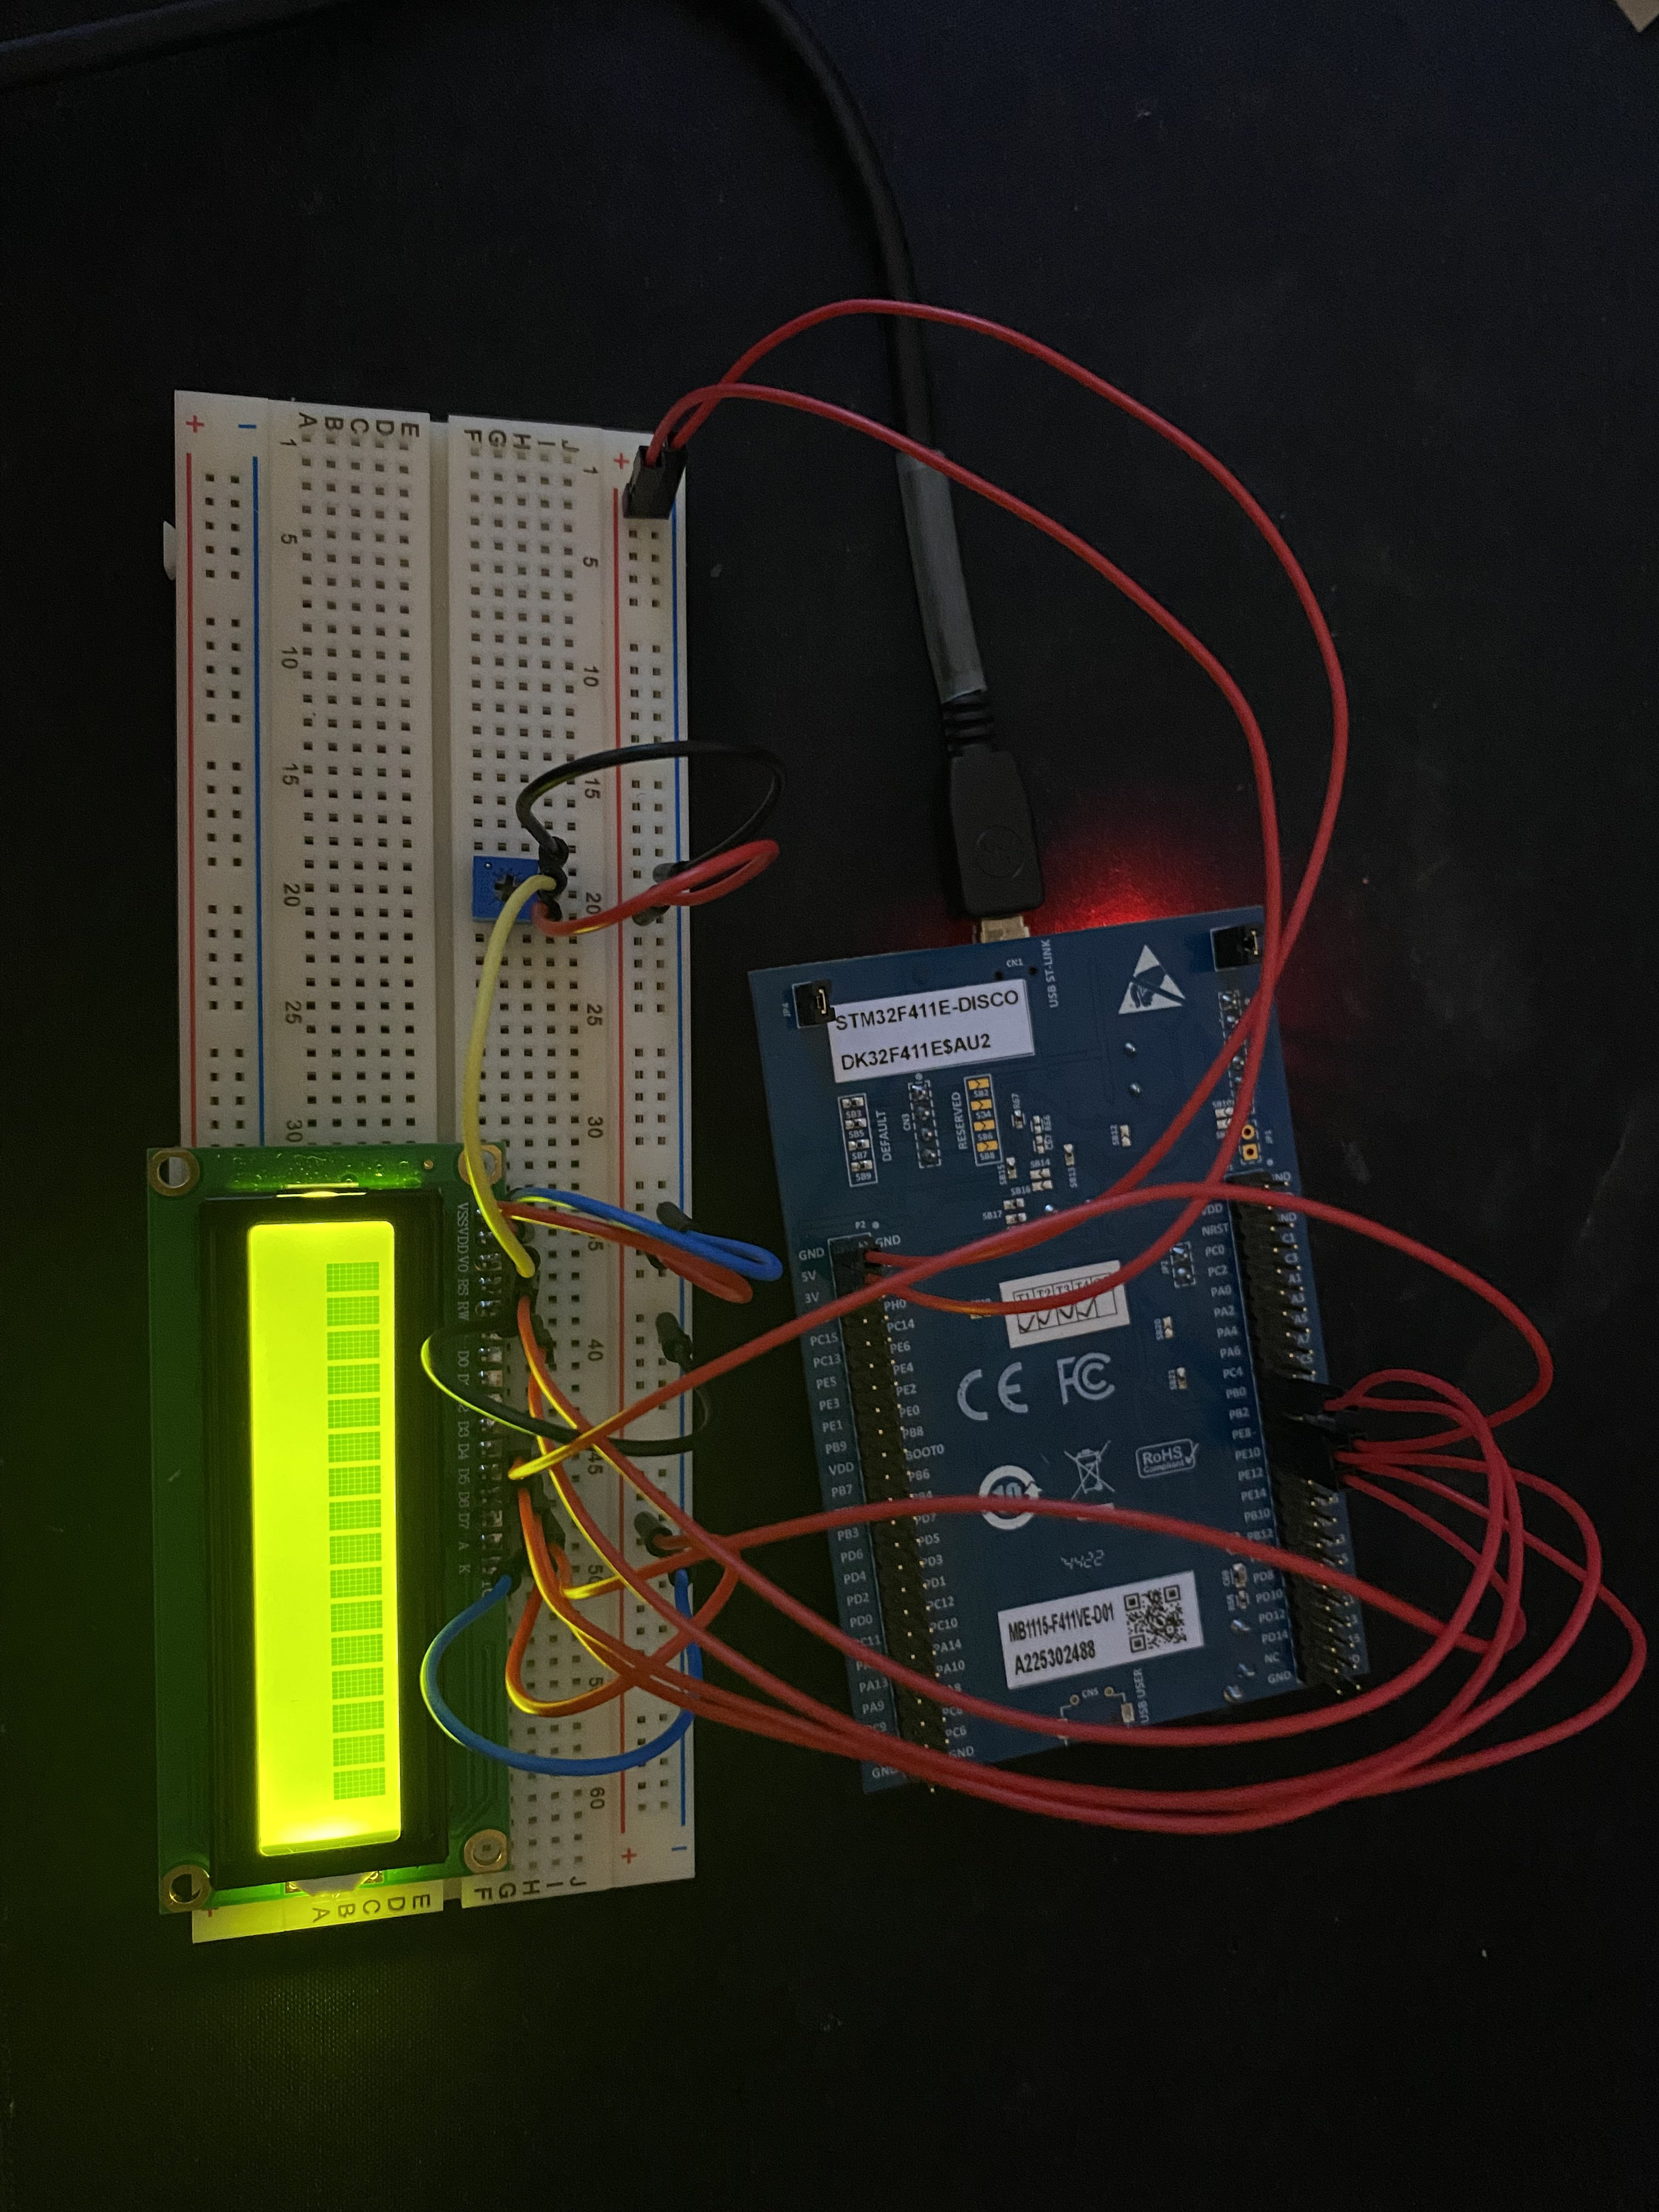
\includegraphics[angle=90,origin=c , width=\linewidth]{images/przed_wlaczeniem.jpg}
}{%
  \caption{Zdjęcie wykonanych połączeń}%
}
\end{figure}

\newpage
\section{Działanie programu}
         Z żyroskopu oraz akcelerometru (wbudowanego w mikrokontroler) przy użyciu odpowiednio interfejsu SPI oraz I2C odczytywane są wartości prędkości kątowej, oraz przyśpieszenia z 3 osi.\\
         
         Następnie na podstawie tych wartości zapisane są odpowiednie warunki na podstawie, których wyświetla się sztuczny horyzont na wyświetlaczu LCD. Obok pokazywane są przeskalowane wartości z żyroskopu. Dodatkowo po przekroczeniu pewnych wartości granicznych żyroskopu, generowany jest sygnał PWM, który może być podany na diodę LED, bądź brzęczyk.\\
        \\
        Kod napisany w języku C, oparty jest o programowanie strukturalne. Wywoływane są funkcje korzystające ze zmiennych globalnych.
        

\section{Użyte funckje}

Do wyświetlania na LCD, została wykorzystana biblioteka, załączona jako lcd.c. Wyświetlanie odbywa się zapomocą 4-bitowej komunikacji GPIO. Jedynie w trybie w trybie write. Bity danych są wysyłane w dwóch połówkach. Korzystając w funkcji lcd\_str\_XY(x,y,str) umiejscawiamy kursor w pozycji x,y i wypisujemy znaki ze zmiennej str.
\\
\\
Obsługując żyroskop i akcelerometr, kluczowa jest ich prawidłowa inicjalizacja. Wykonywane jest to w utworzonych funkcjach, odpowiednio I3G4250D\_init() i LSM303AGR\_init(). Po sprawdzeniu rejestru WHO\_AM\_I, zapisywana jest odpowiednia sekwencja 0 i 1, do rejestru CTRL1. 
\\
\\
Kolejno do odczytu parametrów z żyroskopu została utworzona funkcja I3G4250D\_Read\_Gyro(), która wykorzystując funckję HAL\_SPI... odczytuje kolejno osi x,y,z następnie łączy wartości górnej i dolnej połowy, oraz skaluje do stopni/sekundę.
\\
\\
LSM303AGR\_Read\_Acc(), służąca do odczytu akcelerometru, działa bliźniaczo podobnie do wcześniej opisanej funkcji, z tym że wykorzystuje interfejs I2C, korzystając z funkcji HAL\_I2C...
\\
\\
stall\_signal(), służy do generacji sygnału PWM, na pinie PA3, wykorzystując Timer 2 i Channel 4. Funckcja ta sprawdza czy zaistniał warunek do generacji. Jeśli tak uruchamia PWM, jeżeli odczyt z żyroskopu jest jeszcze większy zmienia wypełnienie sygnału przez zmianę rejestru CCR.
\\
\\
Funkcje inicjalizujące znajdują się w funkcji main, przed pętlą while. Natomiast pozostałe wywoływane są w jej wnętrzu.

\section{Testy działania zbudowanego układu}

        W repozytorium w katalogu $/sprawozdanie\_projekt$ znajduje się film .mp4 prezentujący działanie układu. \\
        
        \begin{figure}[H]
\begin{floatrow}
\ffigbox{%
  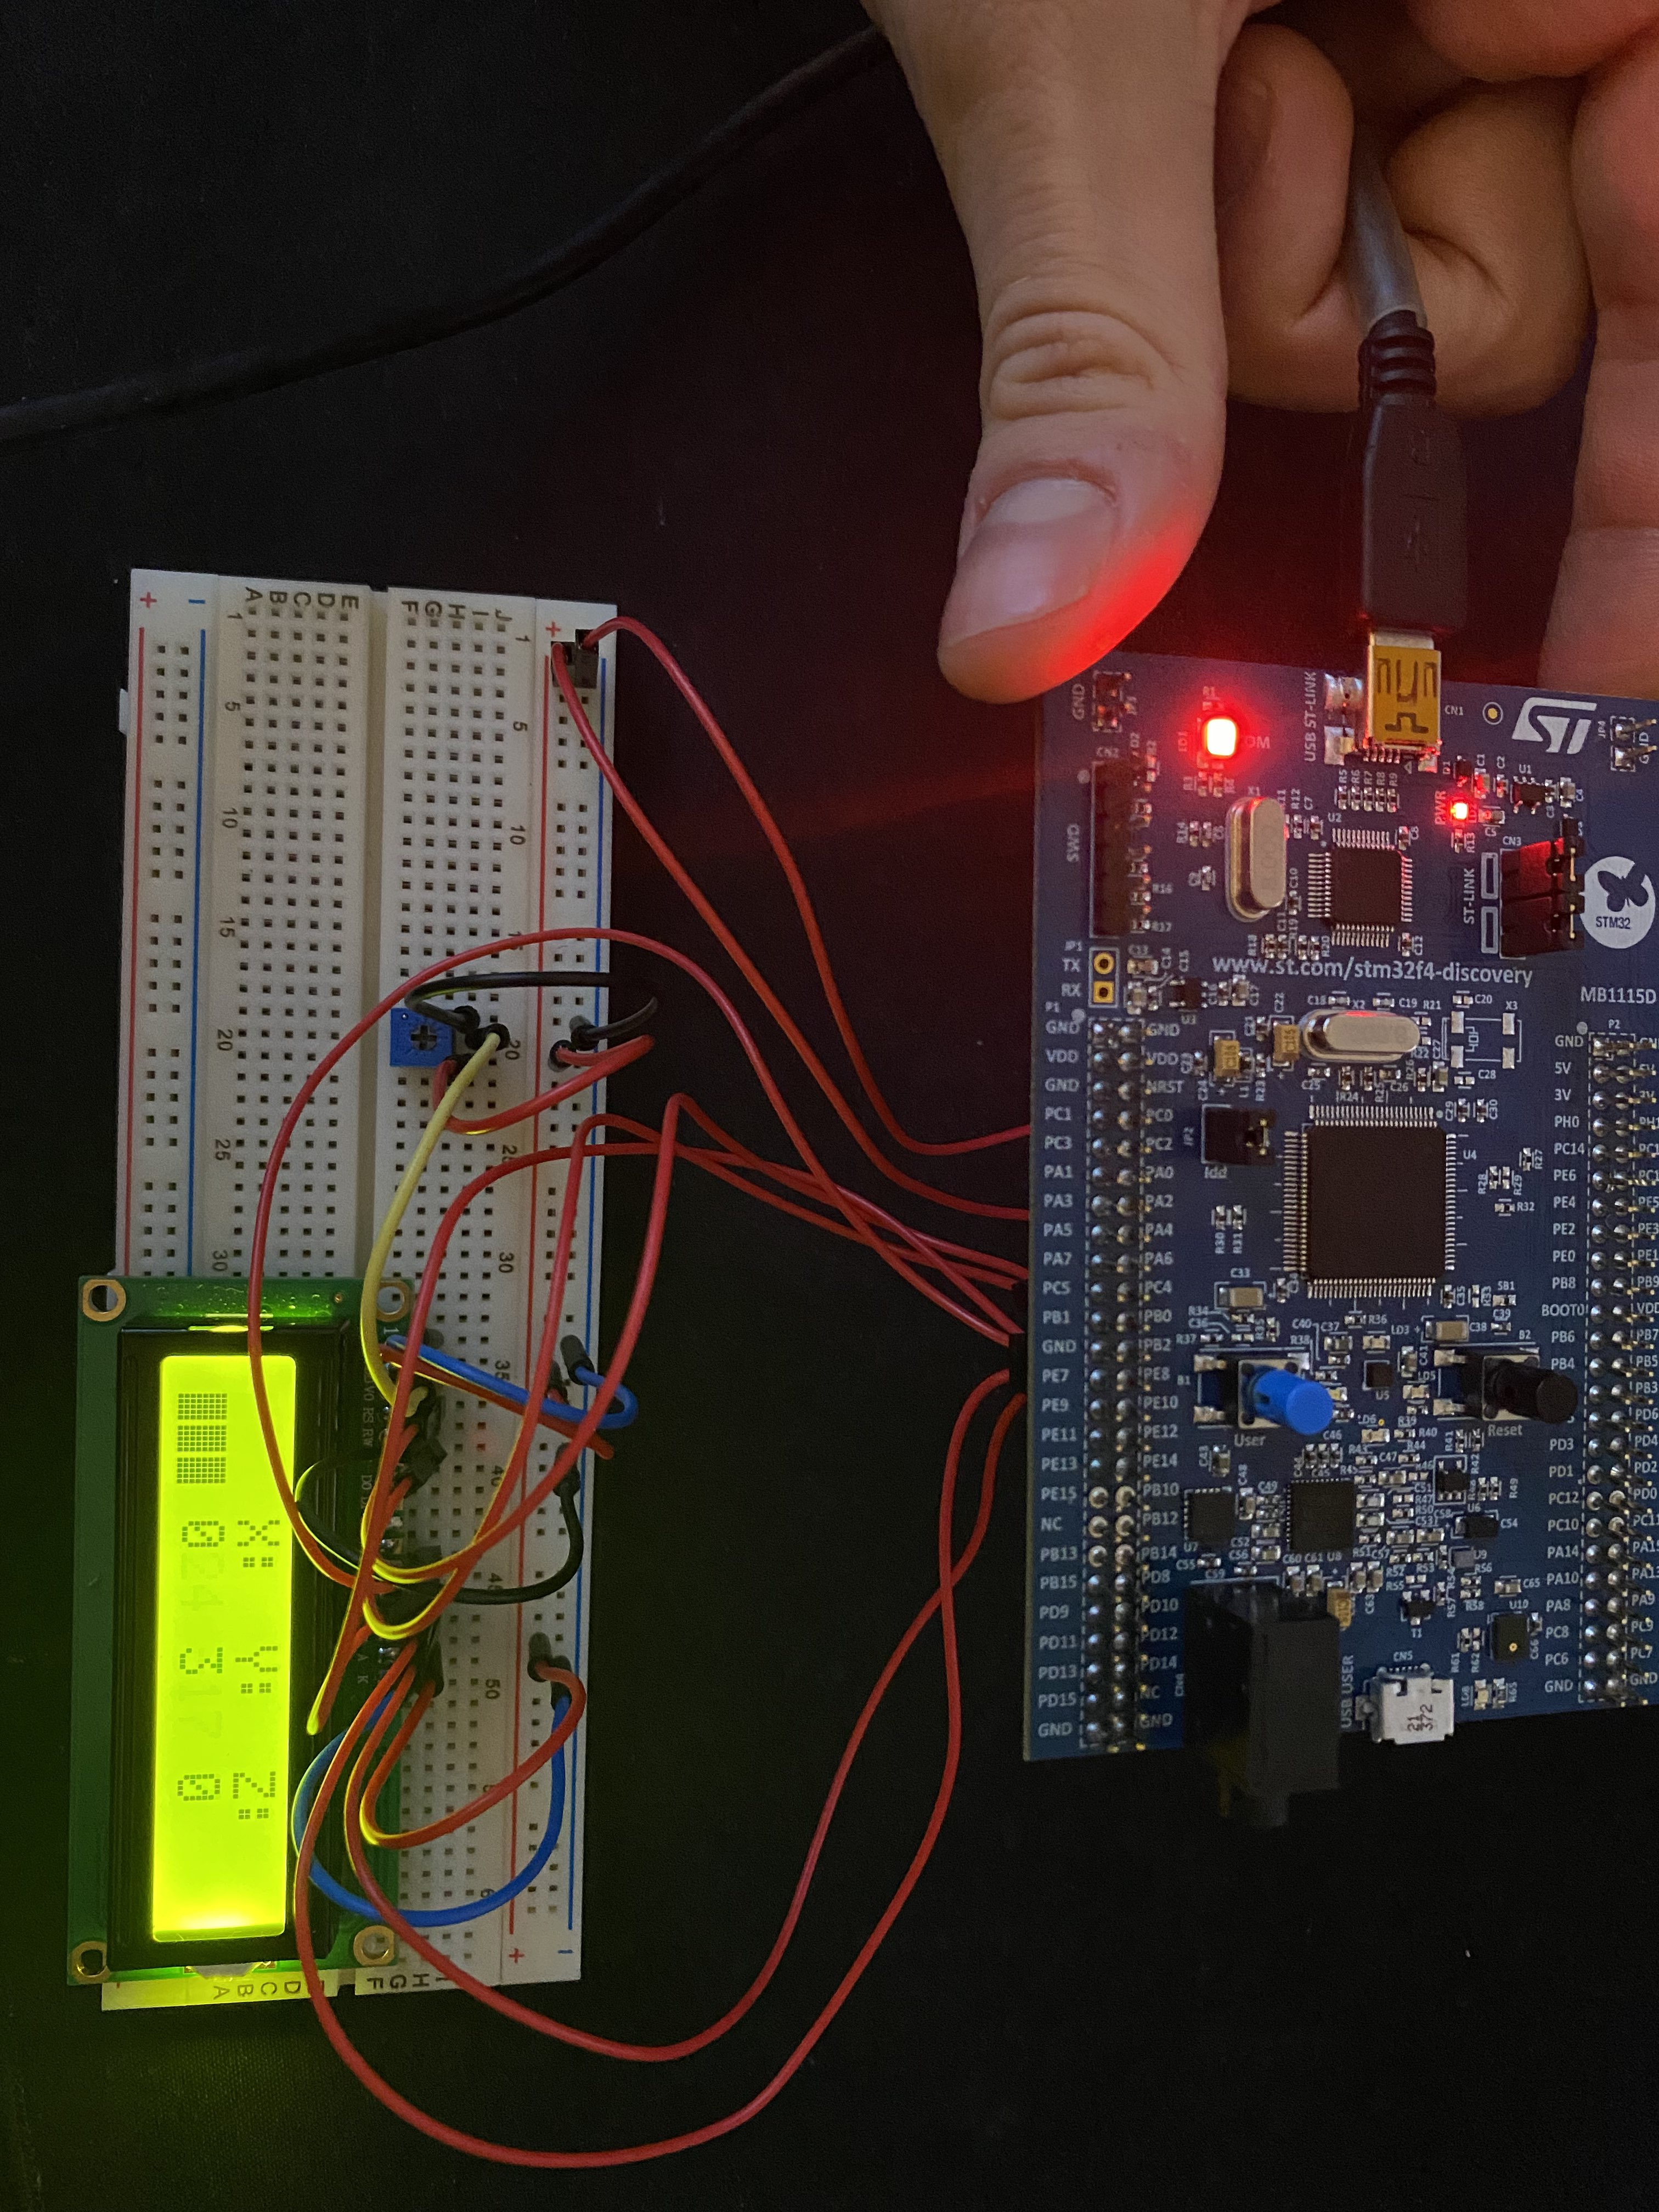
\includegraphics[angle=90,origin=c, width=\linewidth]{images/normalnie.jpg}
}{%
  \caption{Wynik działania w poleżeniu poziomym}%
}
\ffigbox{%
  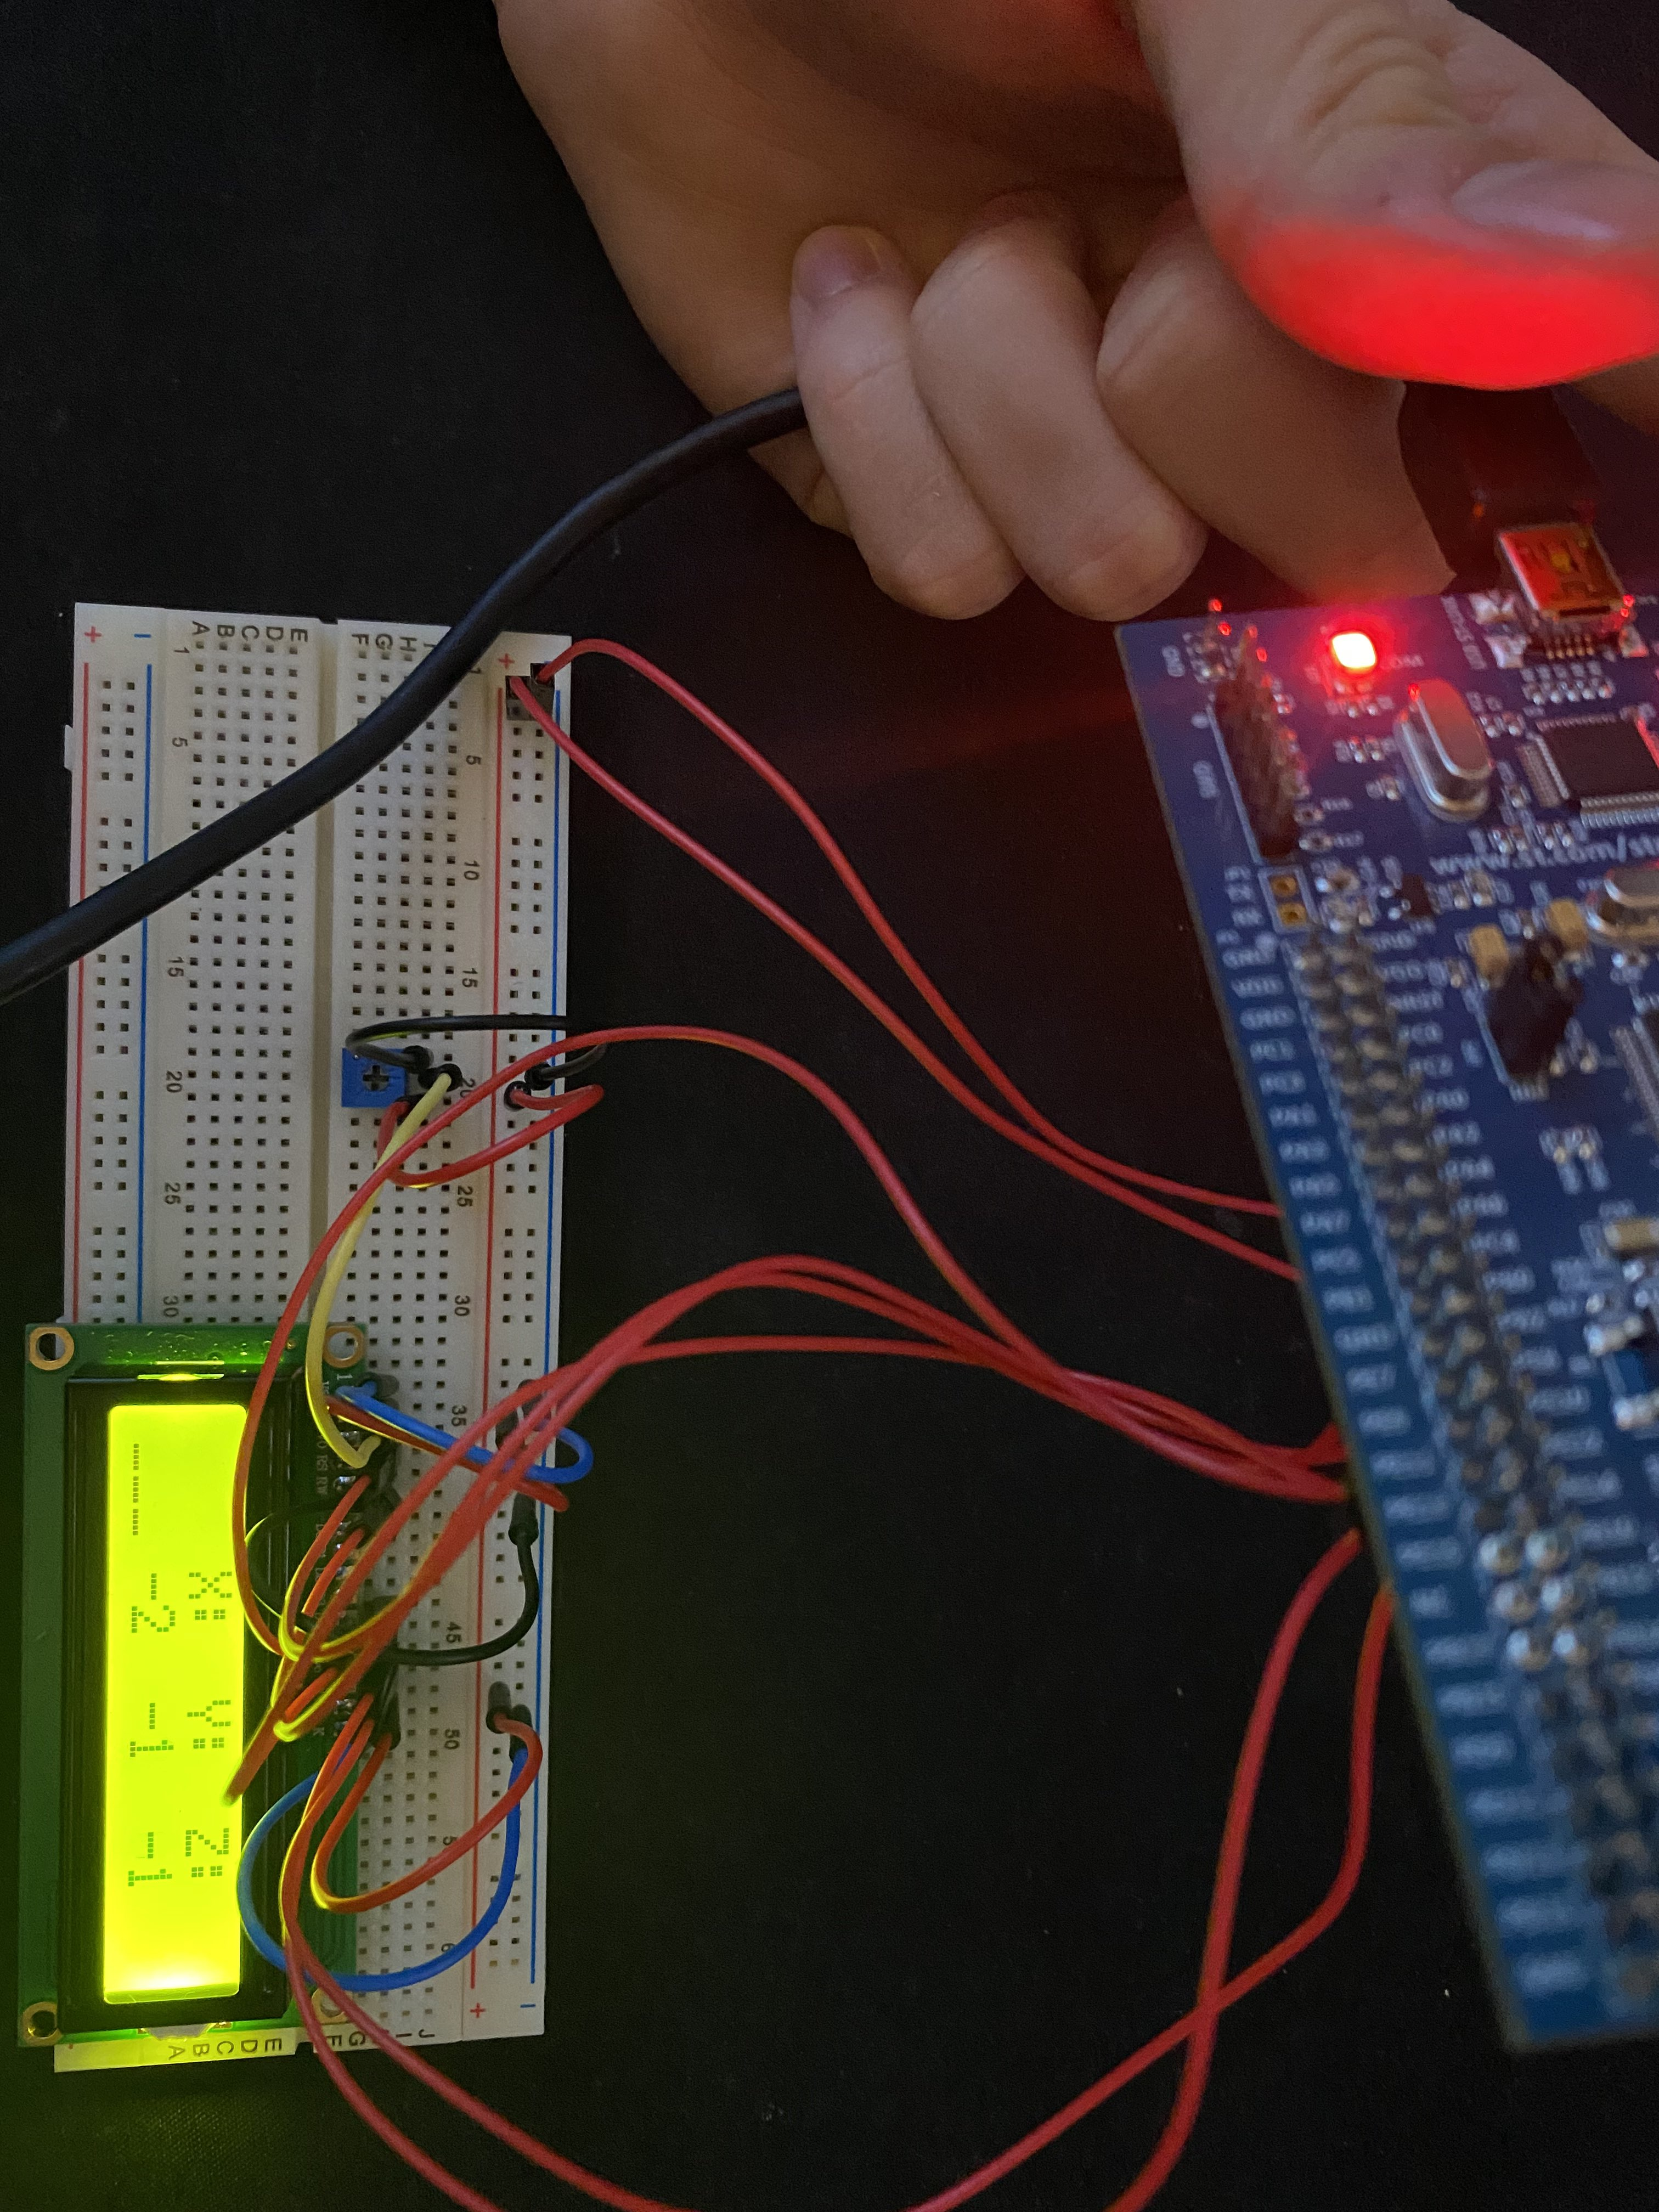
\includegraphics[angle=90,origin=c, width=\linewidth]{images/przechyl_w_tyl.jpg}
}{%
  \caption{Wynik działania w przechyleniu w tył}%
}
\end{floatrow}
\end{figure}

        \begin{figure}[H]
\begin{floatrow}
\ffigbox{%
  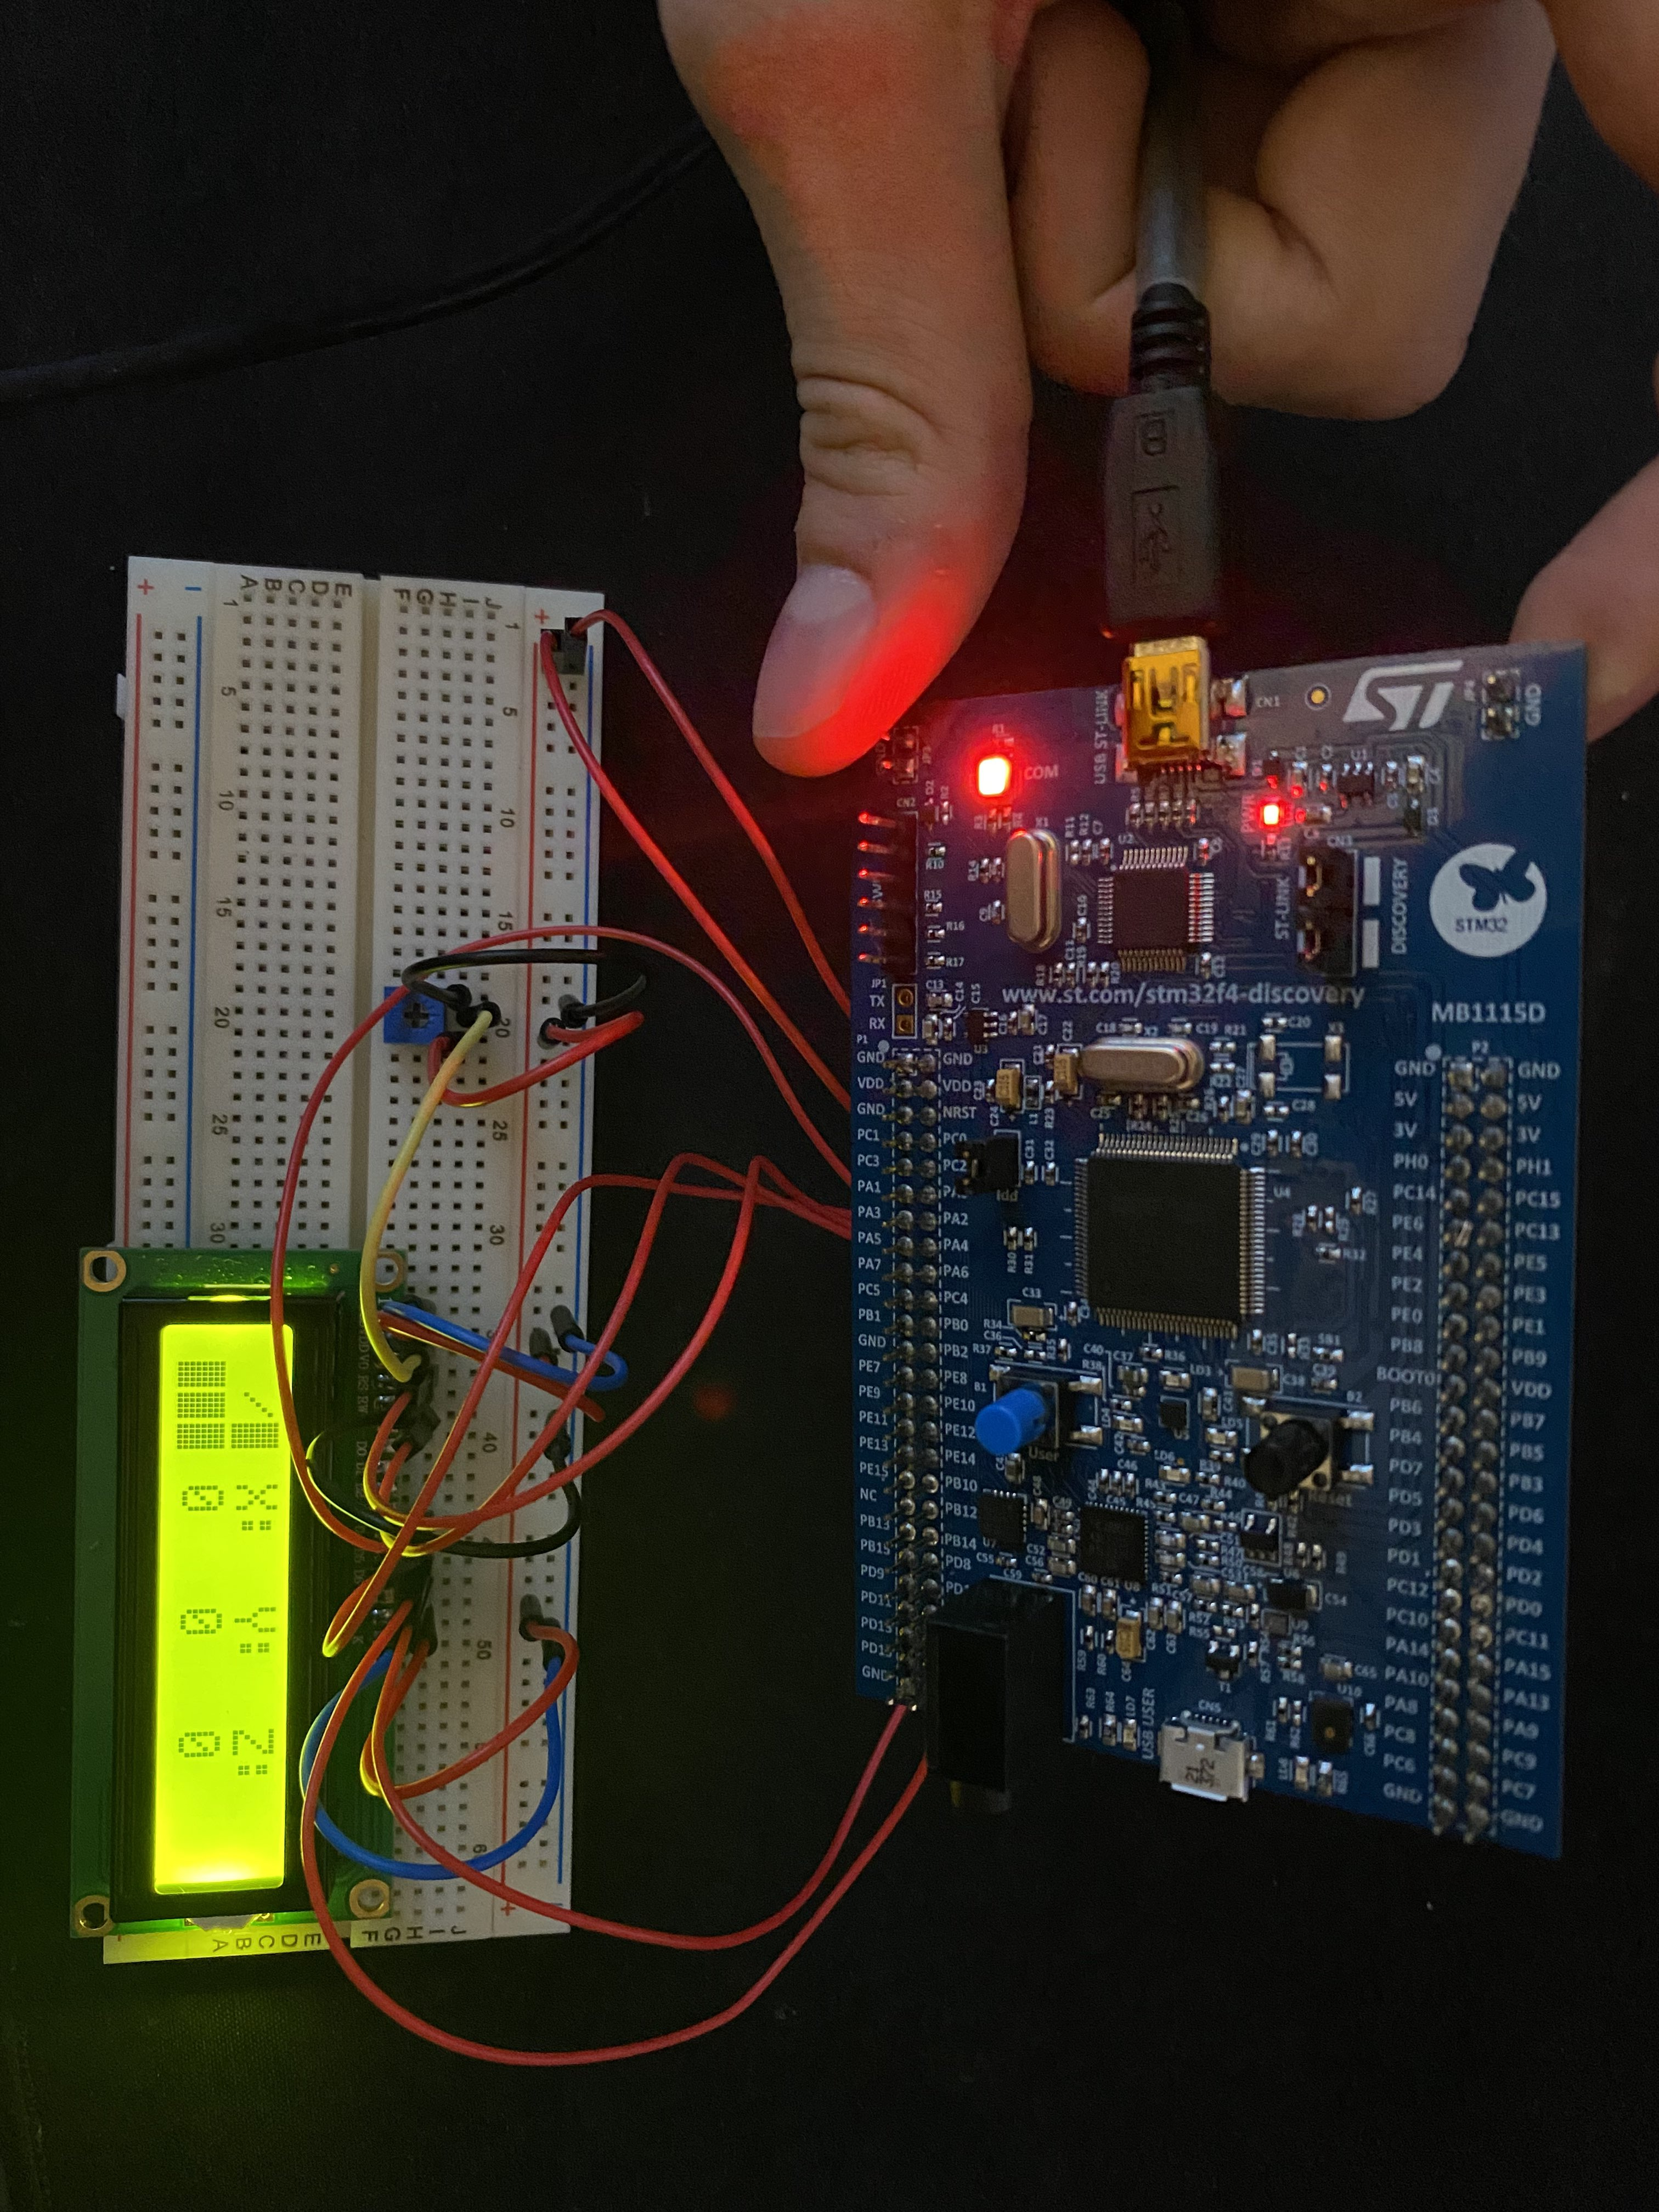
\includegraphics[angle=90,origin=c, width=\linewidth]{images/przechyl_w_prawo.jpg}
}{%
  \caption{Wynik działania w przechyleniu w prawo}%
}
\ffigbox{%
  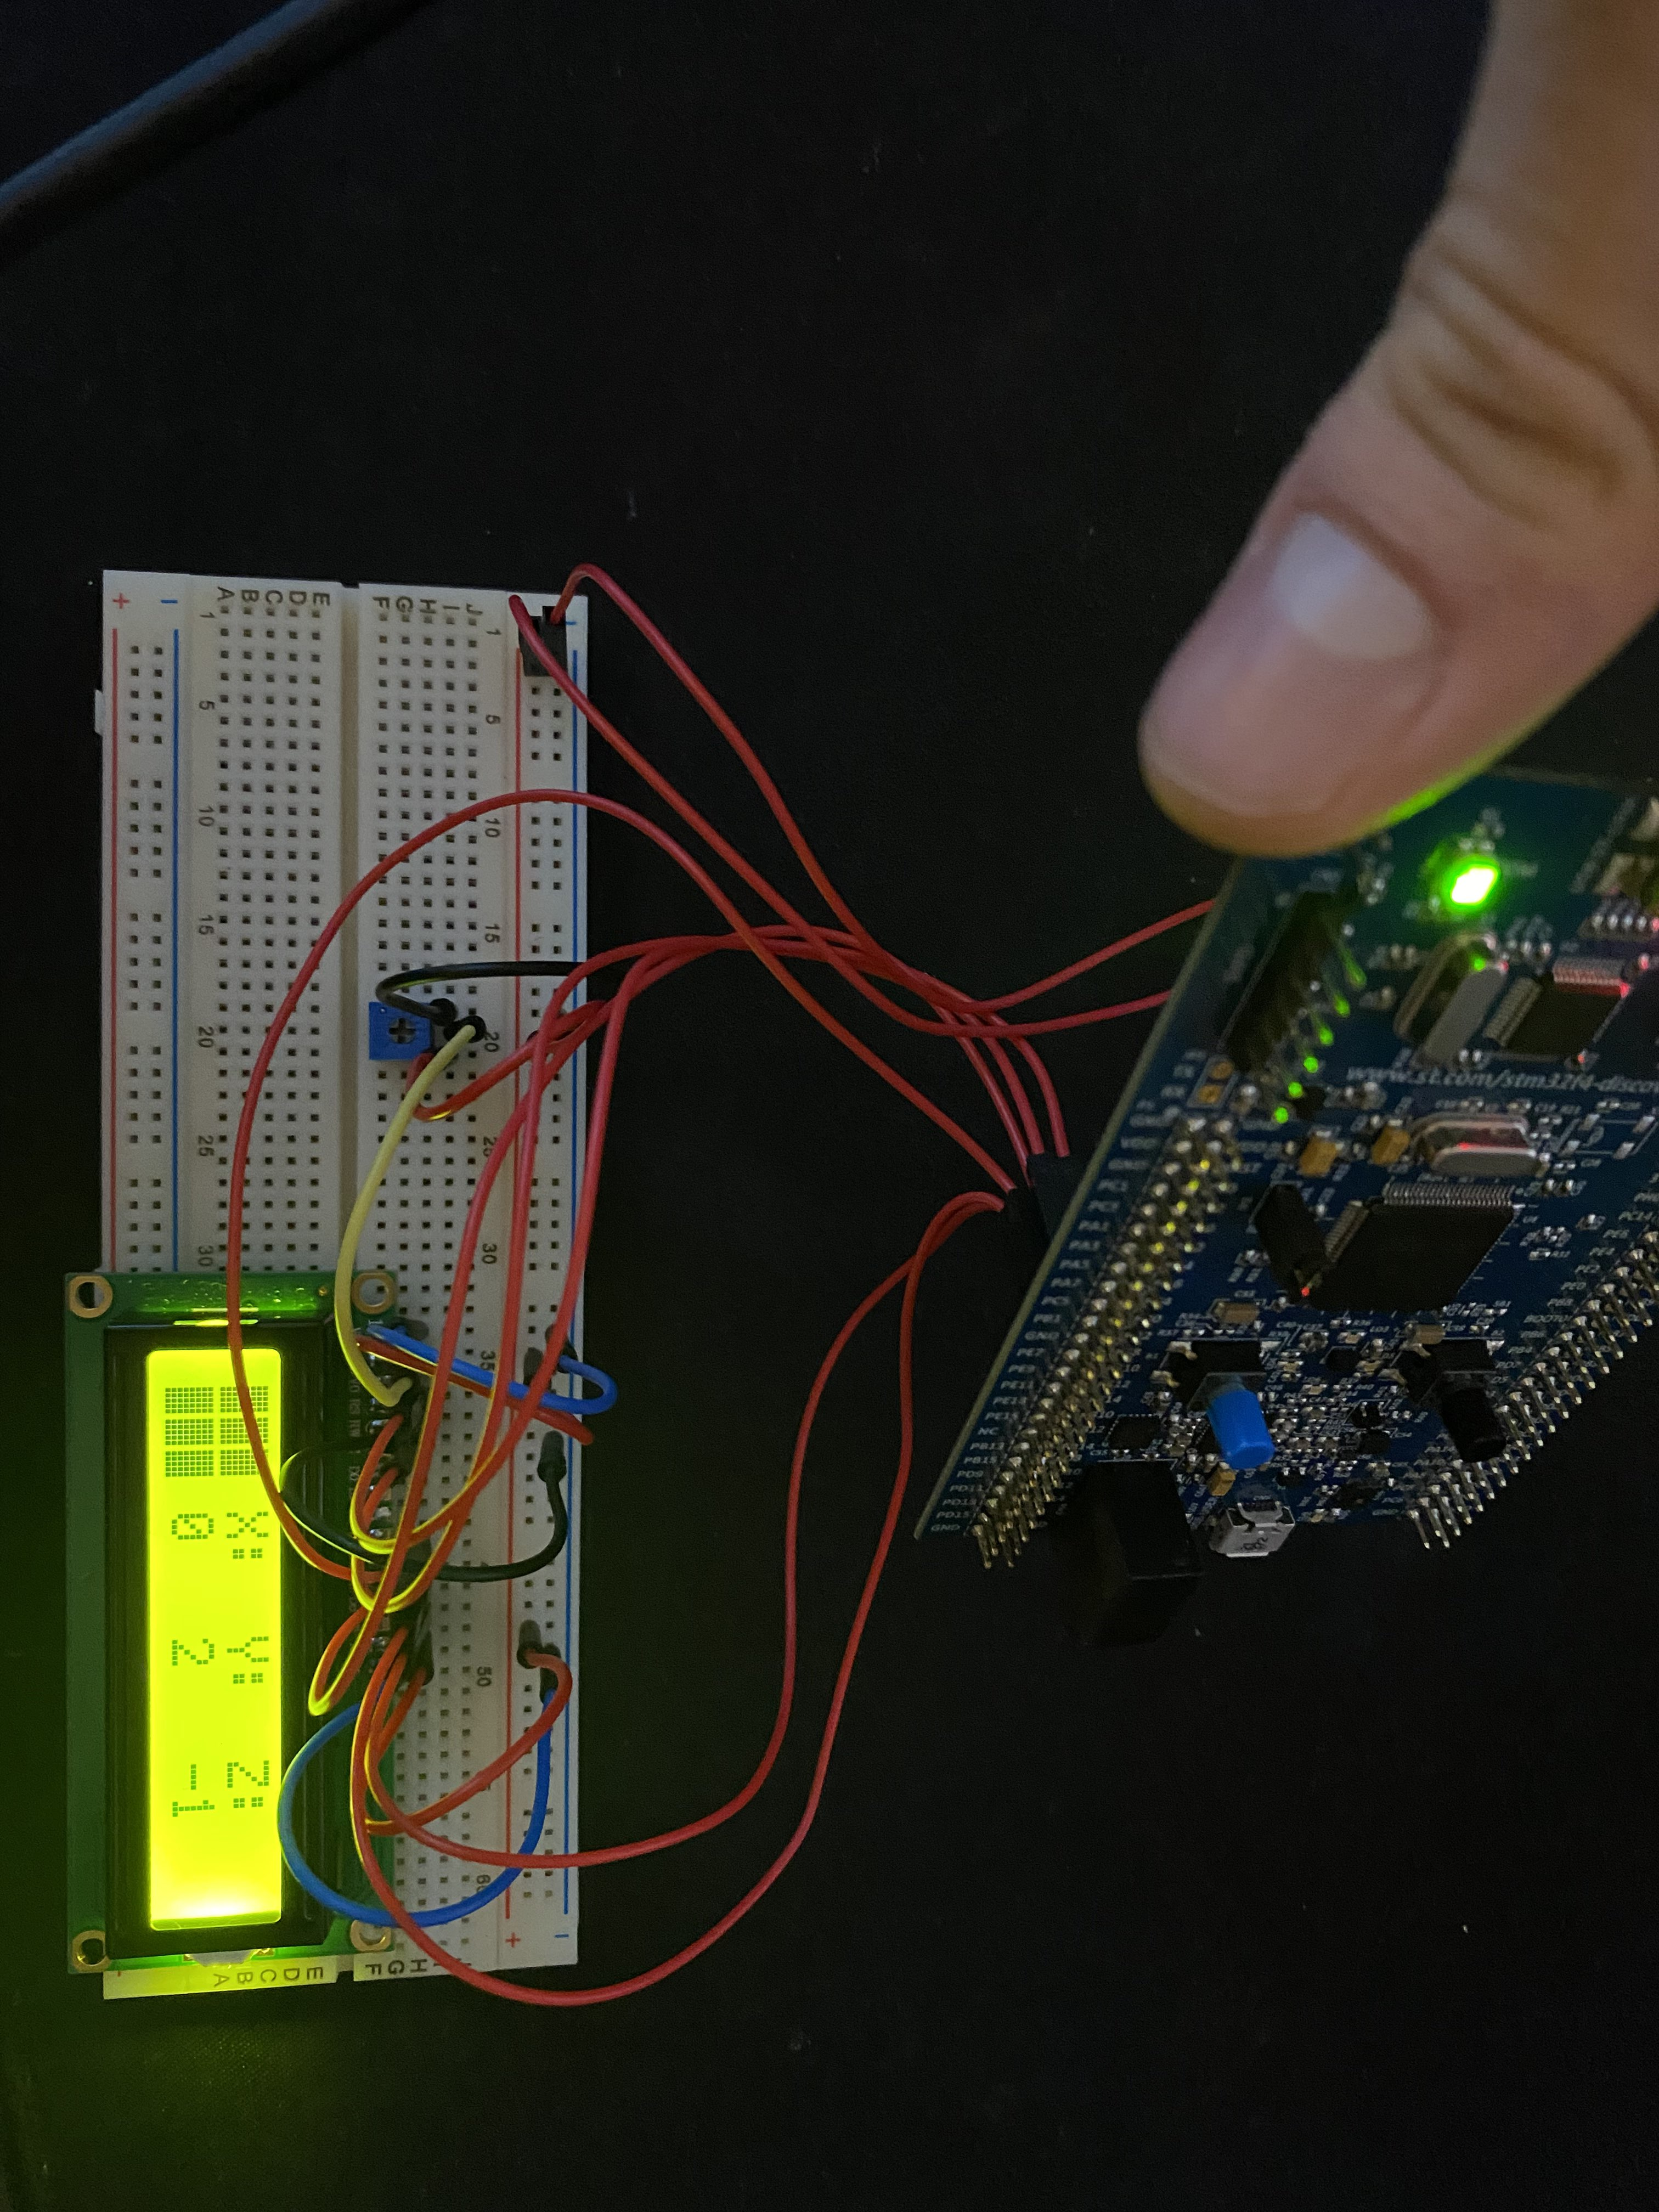
\includegraphics[angle=90,origin=c, width=\linewidth]{images/przechyl_w_przod.jpg}
}{%
  \caption{Wynik działania w przechyleniu w przód}%
}
\end{floatrow}
\end{figure}

Układ działa prawidłowo, zgodnie z oczekiwaniami wyświetlane są symbole, oraz wartości odczytane z żyroskopu.

\section{Wnioski}

Projekt w binarny sposób wyświetla położenie układu. Natomiast odczytane dane z czujników, są poddane jedynie skalowaniu, a nie dalszej analizie, która wymagałaby złożonego powiązania odczytów. Dopiero po tym można by próbować przedstawić szczegółowe informacje o położeniu urządzenia w przestrzeni, a wyświetlacz LCD 16x2 zastąpić lepszym, o większej rozdzielczości.
\\
\\
Wykorzystując ponownie wyświetlacz LCD 16x2, z pewnością wykorzystalibyśmy dodatkowy interfejs umożliwiający komunikację za pomocą I2C, zmniejszyłoby to ilość podpinanych przewodów i uprościłoby pisanie kodu.
\\
\\
Uruchomienie czujników, wymagało wnikliwej analizy dokumentacji, konkretnych modeli czujników. Następnie chcąc przeskalować do rzeczywistych wartości, najszybszym rozwiązaniem okazało się doświadczalne wyznaczenie współczynników skalujących.



\end{document}
